\documentclass{article}
\title{Differentiable Neural Computer Learning Note}
\author{Zhengzhong Liang}
\date{2018-04-30}

\usepackage{hyperref}
\hypersetup{
    colorlinks=true,
    linkcolor=blue,
    filecolor=magenta,      
    urlcolor=cyan,
}

\usepackage[margin=1in]{geometry}
\usepackage{graphicx}
\usepackage[section]{placeins}

\begin{document}
\maketitle
\section{Ultimate Topics to Study}
\subsection{What type of task does this agent try to finish}
\subsection{What is the function of memory in this task}
\subsection{What tyep of tasks can we train the agent to do}
\subsection{What parts and functions can we add to this agent}

\section{Learning Note 20180505}
\subsection{Agent Task Analysis}
\subsubsection{What is the agent trying to learn?}
This agent tries to learn a pattern with timestep 9 and dimension 6 (acoording to the default print result). This pattern is generated by input sequence, which is tensor with shape $9\times16\times6$. So I
\subsubsection{Is there any law used to generate this pattern?} 


\subsection{Experiments}
\subsubsection{Try to pring the sequence of each time step of a single sample in the batch}
The following variables should be printed: input sequence, output sequence of controller, write heads, memory, usage, read heads, access output. {\color{red}refer to paper, use a simple example to figure out how each part is collaberating with other parts}


\section{Code Structure}
\subsection{About Computation Graph}
The basic graph is defined in ``DNC.py'', some peripheral parts of graph is defined in ``run$\_$model''function and ``train.py''. The main parts of computation graph of DNC is organized as following:
\section{Code Features}
\subsection{The Structure of Return Value of DNC Core}
\begin{table}[!htb]
\centering
\caption{The Sructure and Size of State Tuple}
\begin{tabular}{| l | c | c | r |} \hline
Level 1  & Level 2          & Level 3           & Level 4  \\ \hline
DNCState & access$\_$output $(16\times4\times16)$ &                   &   \\ \hline
         & access$\_$state  & memory $(16\times16\times16)$ &   \\ \hline
         &                  & read$\_$weights $(16\times4\times16)$ &   \\ \hline
         &                  & write$\_$weights $(16\times1\times16)$ &   \\ \hline
         &                  & linkage           & link $(16\times1\times16\times16)$ \\ \hline
         &                  &                   & precedence$\_$weights $(16\times1\times16)$ \\ \hline
         &                  & usage $(16\times16)$ & \\ \hline
         & controller$\_$state    & hidden $(16\times64)$ & \\ \hline
         &                  & cell $(16\times64)$ & \\ \hline
\end{tabular}
\label{tab:TupleStructureSize}
\end{table}

\begin{table}[!htb]
\centering
\caption{Important Parameters (from Code)}
\begin{tabular}{| l | c | r |} \hline
item        & value & meaning \\ \hline
hidden size & 64 & The number of neurons of LSTM (controller) \\ \hline
memory size & 16 & the number of memory slots \\ \hline
word size & 16 & the length of each memory slot \\ \hline
num write heads & 1 & the number of write heads \\ \hline
num read heads  & 4 & the number of read heads \\ \hline
\end{tabular}
\end{table}

\begin{table}[!htb]
\centering
\caption{Tensor Size and Explanation}
\begin{tabular}{| l | c | r |} \hline
tensor name & tensor size & explanation \\ \hline
access output & $16\times4\times16$ & batch size, $\#$ of read heads, $\#$ of memory slots \\ \hline
memory & $16\times16\times16$ & batch size, $\#$ of memory slots, slot length \\ \hline
read weights & $16\times4\times16$ & batch size, $\#$ of read heads, $\#$ of memory slots \\ \hline
write heads & $16\times4\times16$ & batch size, $\#$ of writes heads, $\#$ of memory slots \\ \hline
link  &   &   \\ \hline
precedence weights  &   &   \\ \hline
usage  & $16\times16$  & batch size, $\#$ of memory slots \\ \hline
hidden  & $16\times64$  & batch size, $\#$ of LSTM neurons \\ \hline
cell  & $16\times64$  & batch size, $\#$ of LSTM neurons \\ \hline
\end{tabular}
\end{table}

\subsection{The Illustration of DNC (Unrolled by Time)}
\begin{figure}[!htb]
\centering
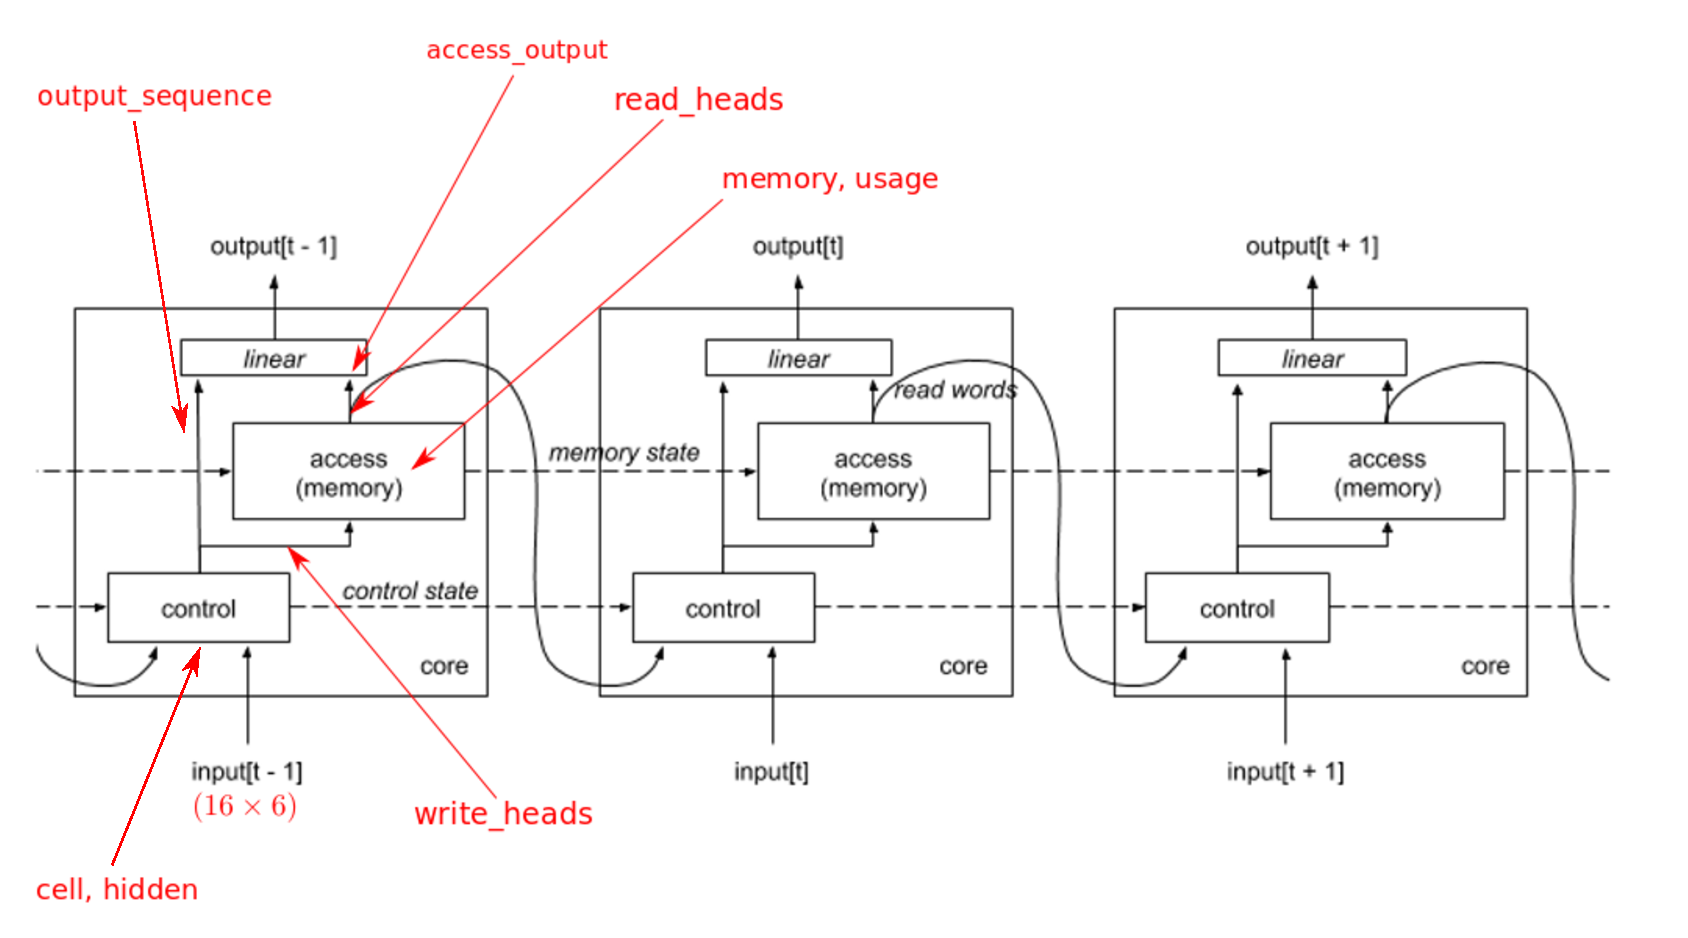
\includegraphics[width=0.98\textwidth]{dnc_model.pdf}
\caption{The Computation Graph of DNC}
\label{fig:DNC_ComputationGraph}
\end{figure}

\section{Question}
\subsection{The memory and controller are defined, but are not connected}
They are connected in the build function, which is called by dynamic rnn function.
\subsection{The build function is not used}
They are used in dynamic rnn function.
\subsection{The functionality of dynamic rnn}
It connects the different parts of the computation graph of DNC, so that a complete graph will be established after calling this function.
\subsection{In every loop a new DNC is created?}
No, the DNC is only built once. 
\subsection{How the computation graph is built in tensorflow?}
Anything before a session starts is considered as computation graph.
\subsection{What does build do in the code}
Connects different parts of computations graph. Build function should be orginally a method of snt.AbstractModule. The abstract module is define 
\href{https://github.com/deepmind/sonnet/blob/master/sonnet/python/modules/base.py}{here}.

As one can see, the build function is a method in this class.
\subsection{Draw UML for the code}
See the UML diagram in the folder.
\subsection{Why there is a init function and a build function in each class}
init function creates the components of the computation graph, while the build function connects these components. The init function is called when the object of DNC is initiated. The build function is called in the tf.nn.dynamic$\_$rnn function.
\subsection{The sequence of calling of build function}
DNC, Access, Freeness, ConsineWeights, TemporalLinkage, ConsineWeights.
\subsection{Draw the inheritance relation ship (and attributes) starting from AbstractModule}
\subsection{Figure out how abstract class works in python (e.g. why no init function)}
Question solved. The method in abstract class can have nothing but a return function. And inherited class can have the method overriding the method in abstract class.

\subsection{Another implementation of DNC}
\href{https://github.com/Mostafa-Samir/DNC-tensorflow/blob/master/dnc/dnc.py}{Is available here}

\subsection{Is the input presented to DNC at each time step?}
Yes the input is presented to DNC at each time step.
\subsection{What is the timestep of DNC}
The timestep of DNC is $9$. That is, the DNC is trying to learning a sequence with length $9$.

\subsection{What is the size of each memory block in DNC memory?}
The memory block is $16\times16$ (16 memory slots, and 16 words each slot).

\section{Questions about DNC}
\subsection{Equivalence between Neural network, Turing machine and brain?}
It is believed that RNN is Turing Complete (Turing complete seems mean that something is equivalent to Turing machine.). And it is believed by some people that brain is not more powerful than Turing machine. So that we can conclude that brain$\neq$RNN$=$Turing Machine.

However, it is questionable then that why we need external memory attacked to RNN if RNN alone is Turing complete.
\end{document}